\chapter{ZAGROŻENIA}
\section{Zagrożenia wynikające z udostępniania danych}

\subsection{Wprowadzenie}

Współczesne organizacje i użytkownicy indywidualni coraz częściej stają się ofiarami zagrożeń wynikających z niekontrolowanego udostępniania danych. Informacje osobiste mogą zostać wykorzystane zarówno przez zewnętrznych atakujących, jak i osoby z wewnątrz firmy — obecnych lub byłych pracowników, kontrahentów, a nawet przypadkowych użytkowników popełniających błędy.
\\
Najczęstsze błędy popełniane przez użytkowników to:
\begin{itemize}
\item publikowanie selfie z oznaczeniem daty i lokalizacji,
\item udostępnianie postów o planowanych lub trwających wyjazdach wakacyjnych,
\item włączona na stałe geolokalizacja w telefonie
\item stosowanie haseł łatwych do odgadnięcia, np. oparte na imionach członków rodziny lub zwierząt, dat urodzin i braku zmiany hasła co jakiś czas,
\item hejtowanie, umieszczanie kontrowersyjnych treści w internecie.
\end{itemize}

Przestępcy mogą wykorzystać te dane do okradzenia mieszkania.
Firmy windykacyjne mogą szybciej ustalić lokalizację użytkownika.
Złodzieje mogą śledzić nawyki i rutynę użytkownika z pomocą danych GPS.\\
Z kolei stworzenie listy kombinacji haseł na podstawie udostępnianych w internecie informacji nie wymaga specjalistycznej wiedzy i pozwala na złamanie hasła w krótkim czasie. Ujawnianie danych osobistych i zwyczajów może prowadzić do łatwego odgadnięcia haseł do kont społecznościowych, bankowości elektronicznej, poczty, czy chmur obliczeniowych. Może to skutkować utratą danych osobistych i prywatnych zasobów, a także podszywanie się pod użytkownika, aby móc wyłudzić informacje lub pieniądze.\\
Kontrowersyjne treści publikowane w internecie mogą skutkować:
\begin{itemize}
  \item Problemami zawodowymi - kontrowersyjne komentarze mogą dotrzeć do pracodawcy.
  \item Pozwem cywilnym - za naruszenie dóbr osobistych innych osób.
  \item Utratą reputacji - zarówno prywatnej, jak i zawodowej.
\end{itemize}

W następnej sekcji przedstawiono opis konkretnych zagrożeń wraz z przykładami z życia codziennego. \cite{zagrozeniaFirmy, zagrozeniaLudzie}

\subsection{Kradzież tożsamości}
\subsubsection{Opis zagrożenia}
Udostępnienie danych osobowych, takich jak imię, nazwisko, PESEL, numer dowodu czy adres e-mail, może skutkować:
\begin{itemize}
\item podszywaniem się pod ofiarę w celu zaciągnięcia pożyczki, otwarcia konta bankowego czy przeprowadzenia transakcji,
\item wykorzystaniem danych w oszustwach ubezpieczeniowych, zdrowotnych lub podatkowych,
\item długoterminowymi problemami finansowymi i prawnymi ofiary.
\end{itemize}
\subsubsection{Przykłady z życia}
W ataku na Marriott w 2020 r. wyciekło ponad 5 mln rekordów gości, zawierających dane kontaktowe, urodziny i numery kont lojalnościowych.\\

5 maja 2020 roku w internecie błędnie zidentyfikowano CEO firmy Propine, Tuhinę Singh, jako kobietę z Singapuru, która została aresztowana po tym, jak w viralowym nagraniu odmówiła założenia maseczki w miejscu publicznym.
W wyniku pomyłki internauci zaczęli publikować jej zdjęcia, numer telefonu, prywatny adres e-mail oraz dane jej współpracowników, co doprowadziło do fali gróźb i rasistowskich obelg.
Skala nagonki była na tyle duża, że firma Propine wydała oficjalne oświadczenie, w którym wyjaśniła, że doszło do pomyłki, a prawdziwa sprawczyni została już zidentyfikowana i odpowiednio ukarana przez władze.

\subsection{Naruszenie prywatności i poufności danych}
\subsubsection{Opis zagrożenia}
Dane, które zostaną ujawnione - nawet nieświadomie - mogą naruszyć prywatność pracowników, klientów czy partnerów biznesowych. Skutki to:
\begin{itemize}
\item utrata kontroli nad własnymi informacjami,
\item możliwość ich dalszego rozpowszechniania,
\item narażenie na nieautoryzowane monitorowanie.
\end{itemize}
\subsubsection{Przykłady z życia}
Zdeanonimizowanie konta dyrektora FBI na Twitterze na podstawie danych o obserwujących i członkach rodziny\\
Zidentyfikowanie tajnych baz wojskowych i osób w nich przebywających na podstawie map ciepła portalu Strava\\
Były pracownik Tesli w 2023 r. ujawnił dane ponad 75 000 pracowników, w tym numery SSN i informacje finansowe.\\

W kwietniu 2020 roku w Meridian (Idaho) policjant aresztował kobietę, która odmówiła opuszczenia zamkniętej części parku publicznego. Ograniczenie było związane z lockdownem COVID-19. Inne części parku pozostały otwarte.
Po nagłośnieniu sprawy, libertariańska organizacja Idaho Freedom Foundation opublikowała na Facebooku imię, nazwisko i zdjęcie funkcjonariusza, wzywając ludzi, by „dali znać departamentowi policji w Meridian, co o tym sądzą”.
Dodatkowo, lider grupy Ammon Bundy rozpowszechnił adres domowy policjanta, m.in. wysyłając go na listę mailingową i zapisując na tablicy podczas spotkania grupy. Nagranie z widocznym adresem obejrzano ponad 1200 razy.
Bundy wcześniej twierdził, że „jeśli prawa jakiejś osoby są łamane, tysiące ludzi powinno ją otoczyć, nagłośnić sprawę i pociągnąć sprawców do odpowiedzialności”. Wypowiadał się też za obecnością broni na protestach, mówiąc: „Pierwsza poprawka jest chroniona przez drugą”.
W wyniku ujawnienia danych osobowych, przed domem policjanta zebrały się dziesiątki protestujących, żądając, by przyjął 13-stronicową skargę.
Republikański poseł z Idaho, Greg Chaney, skomentował, że działania Bundy'ego naraziły policjanta i jego rodzinę na poważne zagrożenie i ryzyko.

\begin{figure}
  \centering
  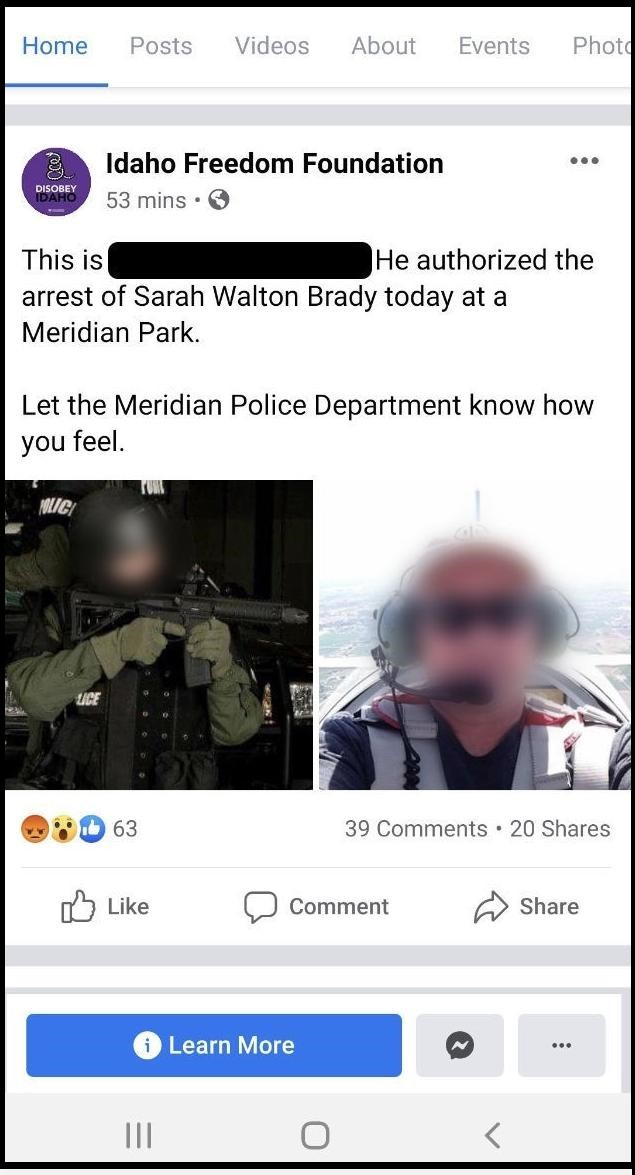
\includegraphics[width=1\textwidth]{images/officer.jpg}
  \caption{Post na Facebooku}
  \label{fig:officer}
\end{figure} 

W marcu 2025 roku w Niebezpieczniku\cite{empik} pojawiło się ogłoszenie dotyczące sprzedaży rzekomej bazy danych zawierającej informacje o 24 milionach klientów Empiku. Zgodnie z opisem, baza miała zawierać takie dane jak: imię i nazwisko, numer telefonu, adres (zamieszkania lub dostawy), adres e-mail oraz informacje o zamówieniach (ich liczba i daty). Co istotne, w ogłoszeniu oraz w udostępnionej próbce danych nie znalazły się żadne hasła ani ich hashe.
Pojawiły się jednak wątpliwości co do autentyczności i pochodzenia danych - m.in. podejrzanie wysoka liczba rekordów (24 mln), która mogła wynikać z błędnego formatowania (sugerowano, że mogło chodzić o 2,4 mln). Sugerowano również, że źródłem danych może być nie Empik, lecz zewnętrzny system reklamowy lub trackingowy, który mógł generować duplikaty.\\
Empik zareagował na incydent, publikując oświadczenie, w którym poinformował, że:
\begin{itemize}
  \item większość danych z próbki nie występuje w ich systemach,
  \item format danych różni się od stosowanego w systemach wewnętrznych firmy,
  \item część ujawnionych informacji to ogólnodostępne dane produktowe z katalogu Empik.com,
  \item nie doszło do wycieku haseł, historii zakupów ani danych płatniczych,
  \item zgodnie z normą PCI DSS firma nie przechowuje numerów kart płatniczych.
\end{itemize}

Zalecano klientom zachowanie ostrożności i zmianę hasła na wypadek, gdyby dane jednak pochodziły z realnego wycieku i przypomniano, że na podstawie danych takich jak nazwisko, e-mail, adres czy numer telefonu można wzajemnie ustalić inne informacje o osobie.
Aktualizacja z 23 marca 2025 roku przyniosła kolejne, kluczowe oświadczenie Empiku: po szczegółowej analizie stwierdzono jednoznacznie, że rzekoma baza danych była fałszywa i została spreparowana na podstawie danych pochodzących z historycznych wycieków z innych firm, najprawdopodobniej w celu oszukania potencjalnych kupujących.
Empik zapewnił, że nie doszło do żadnego incydentu bezpieczeństwa po ich stronie, dane klientów są bezpieczne, a firma natychmiast po pojawieniu się sygnałów o możliwym wycieku uruchomiła proces weryfikacji z pomocą zespołu CERT. Firma również przestrzegła przed powielaniem niezweryfikowanych informacji dotyczących bezpieczeństwa danych.
W tym przypadku było to akurat fałszywe ogłoszenie, ale bardzo ważne jest by firmy reagowały właściwymi działaniami na tego typu incydenty, tak jak zrobiła to firma Empik.

\begin{figure}
  \centering
  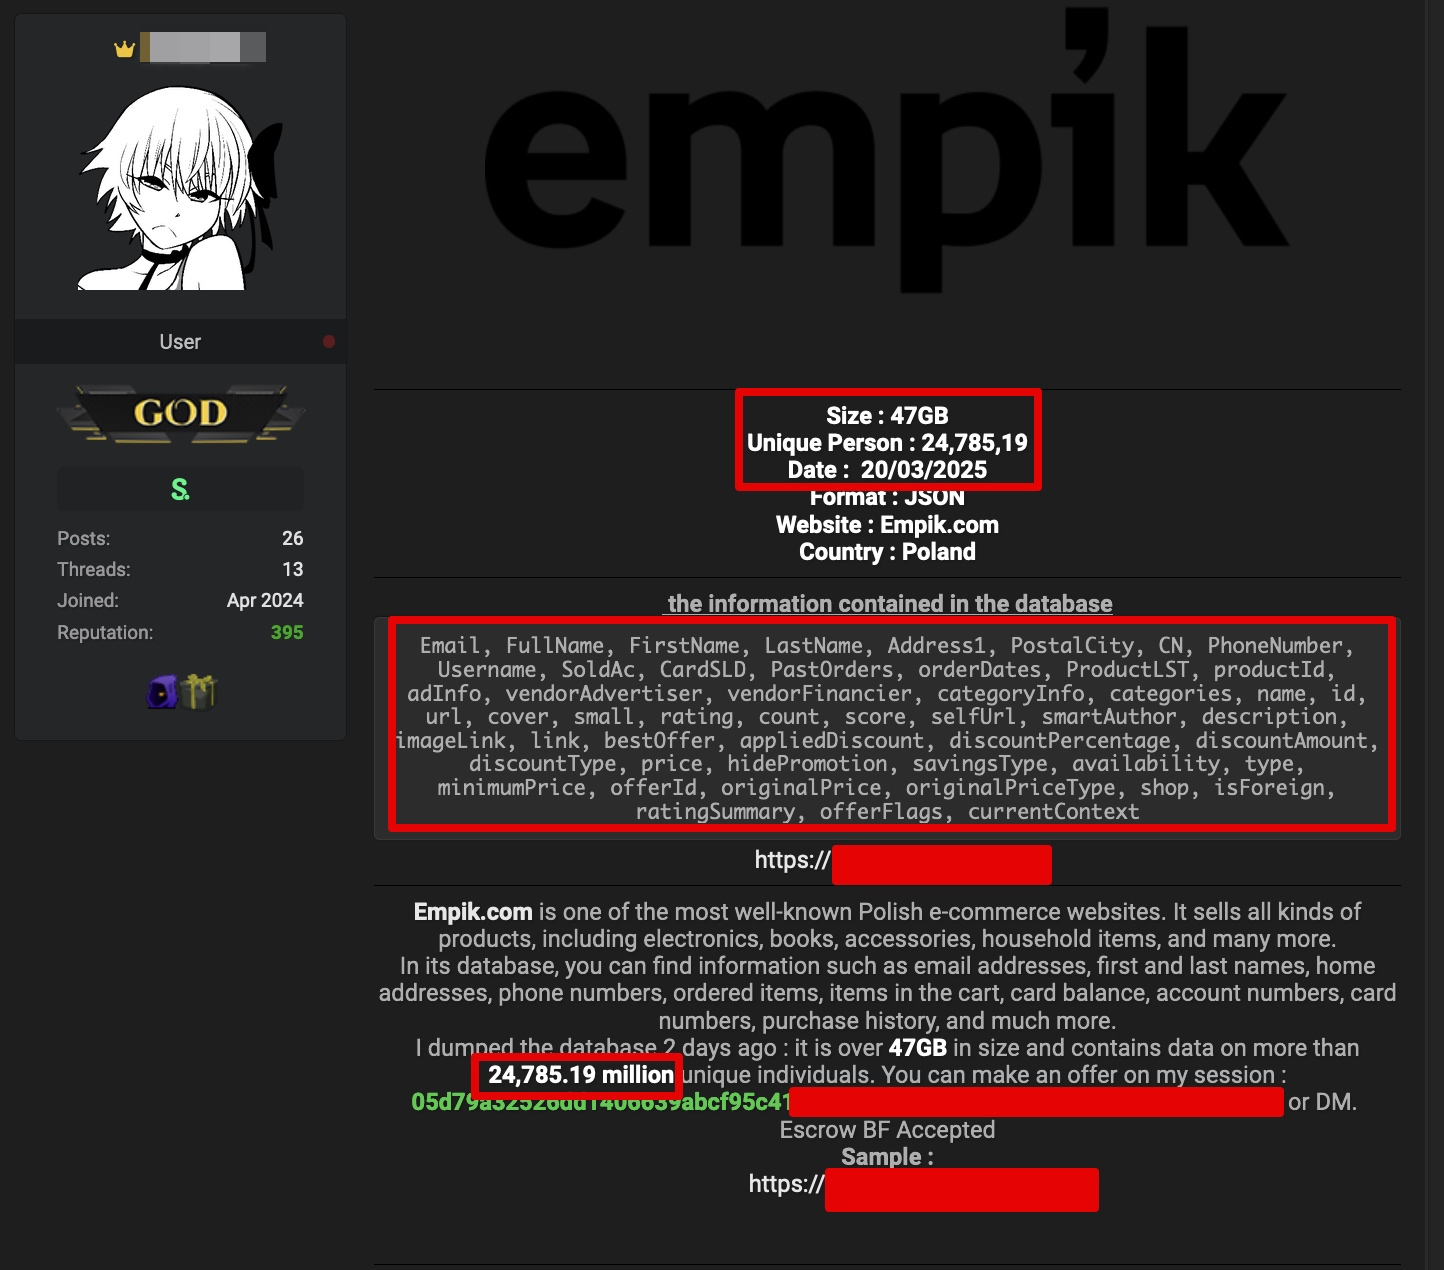
\includegraphics[width=1\textwidth]{images/empik-wyciek.jpg}
  \caption{Ogłoszenie sprzedaży bazy danych klientów empiku}
  \label{fig:empik}
\end{figure} 

\begin{figure}
  \centering
  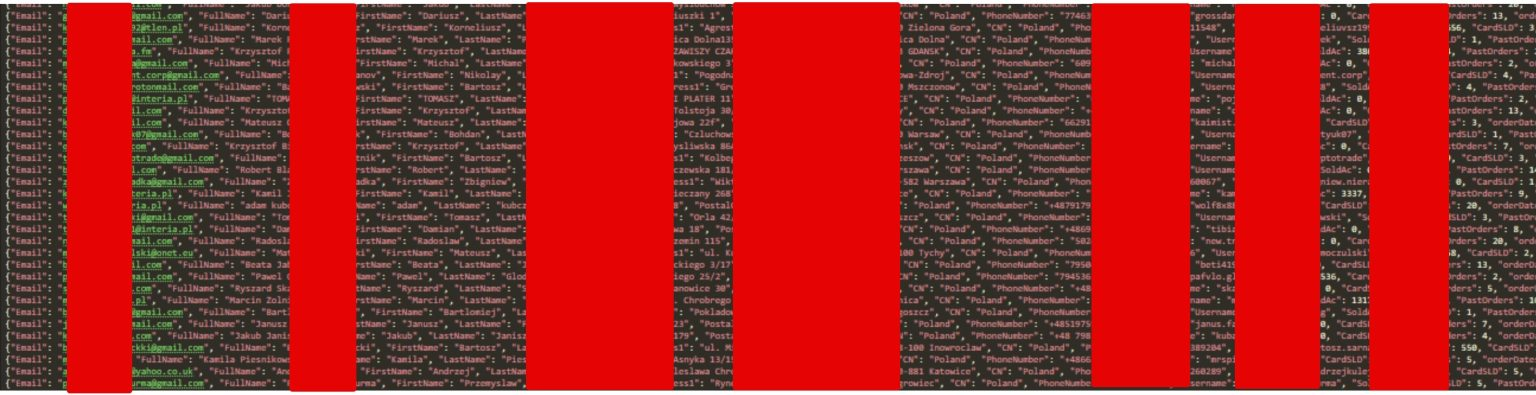
\includegraphics[width=1\textwidth]{images/probka.jpg}
  \caption{Próbka ogłoszenia}
  \label{fig:probka}
\end{figure} 

\subsection{Cyberstalking i nękanie}
\subsubsection{Opis zagrożenia}
Gdy dane kontaktowe lub lokalizacyjne stają się publiczne, rośnie ryzyko:
\begin{itemize}
\item śledzenia i nękania w sieci lub w świecie rzeczywistym,
\item stosowania szantażu lub gróźb,
\item prób kontaktu ze strony osób niepożądanych, np. stalkerów.
\end{itemize}
\subsubsection{Przykłady z życia}
Angela Dunn to epidemiolog nękana przez protestujących, po tym jak opublikowano ulotki z jej adresem na Facebooku, protestujący pojawili się pod jej domem, oskarżając ją o zniszczenie gospodarki przez lockdown. 

\begin{figure}
  \centering
  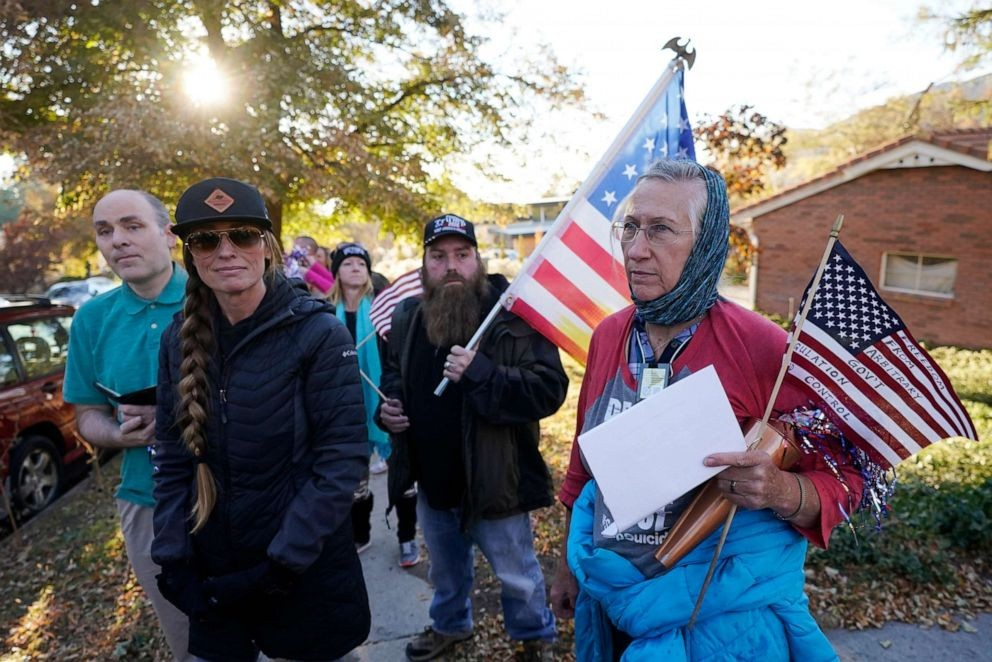
\includegraphics[width=1\textwidth]{images/lockdown.jpg}
  \caption{Protesty pod domem Angeli Dunn}
  \label{fig:lockdown}
\end{figure} 

Laurie Jones, czyli  urzędniczka zdrowia publicznego znalazła się pod ostrzałem gróźb. Po kontakcie z osobą zakażoną COVID-19, gdzie kobieta zadzwoniła do osoby zakażonej, aby przypomnieć jej o tym by została w domu, chociaż zakażona osoba tego nie przestrzegała. Pojawiły się później w internecie pod jej adresem fałszywe oskarżenia o szpiegostwo, szerzenie paniki, co wywołało falę hejtu i groźby śmierci.
Kobieta doświadczyła traumy, musiała zainstalować zabezpieczenia w domu. Do dziś ma obawy przed wychodzeniem z domu i stała się chorobliwie zachowawcza.\\

W styczniu 2021 roku senator Mitch McConnell spotkał się z falą krytyki po tym, jak zablokował propozycję zwiększenia kwoty wypłat w ramach rządowej pomocy COVID-19. W odpowiedzi, niektórzy oburzeni obywatele odnaleźli jego domowy adres i dokonali aktu wandalizmu na jego drzwiach pojawił się napis „Gdzie są moje pieniądze?”, a na ganku umieszczono wulgarne hasła.
Protest został zorganizowany przez grupę DC Under Siege, która opublikowała wydarzenie na Facebooku. Rankiem przed domem senatora zebrała się grupa demonstrantów wyposażonych w megafony i transparenty.
McConnell odniósł się do zajścia, podkreślając, że docenia prawo obywateli do udziału w procesie demokratycznym, również tych, którzy się z nim nie zgadzają. Jednocześnie stanowczo potępił akty wandalizmu i zastraszania, stwierdzając, że „polityka strachu nie ma miejsca w naszym społeczeństwie”.

\begin{figure}
  \centering
  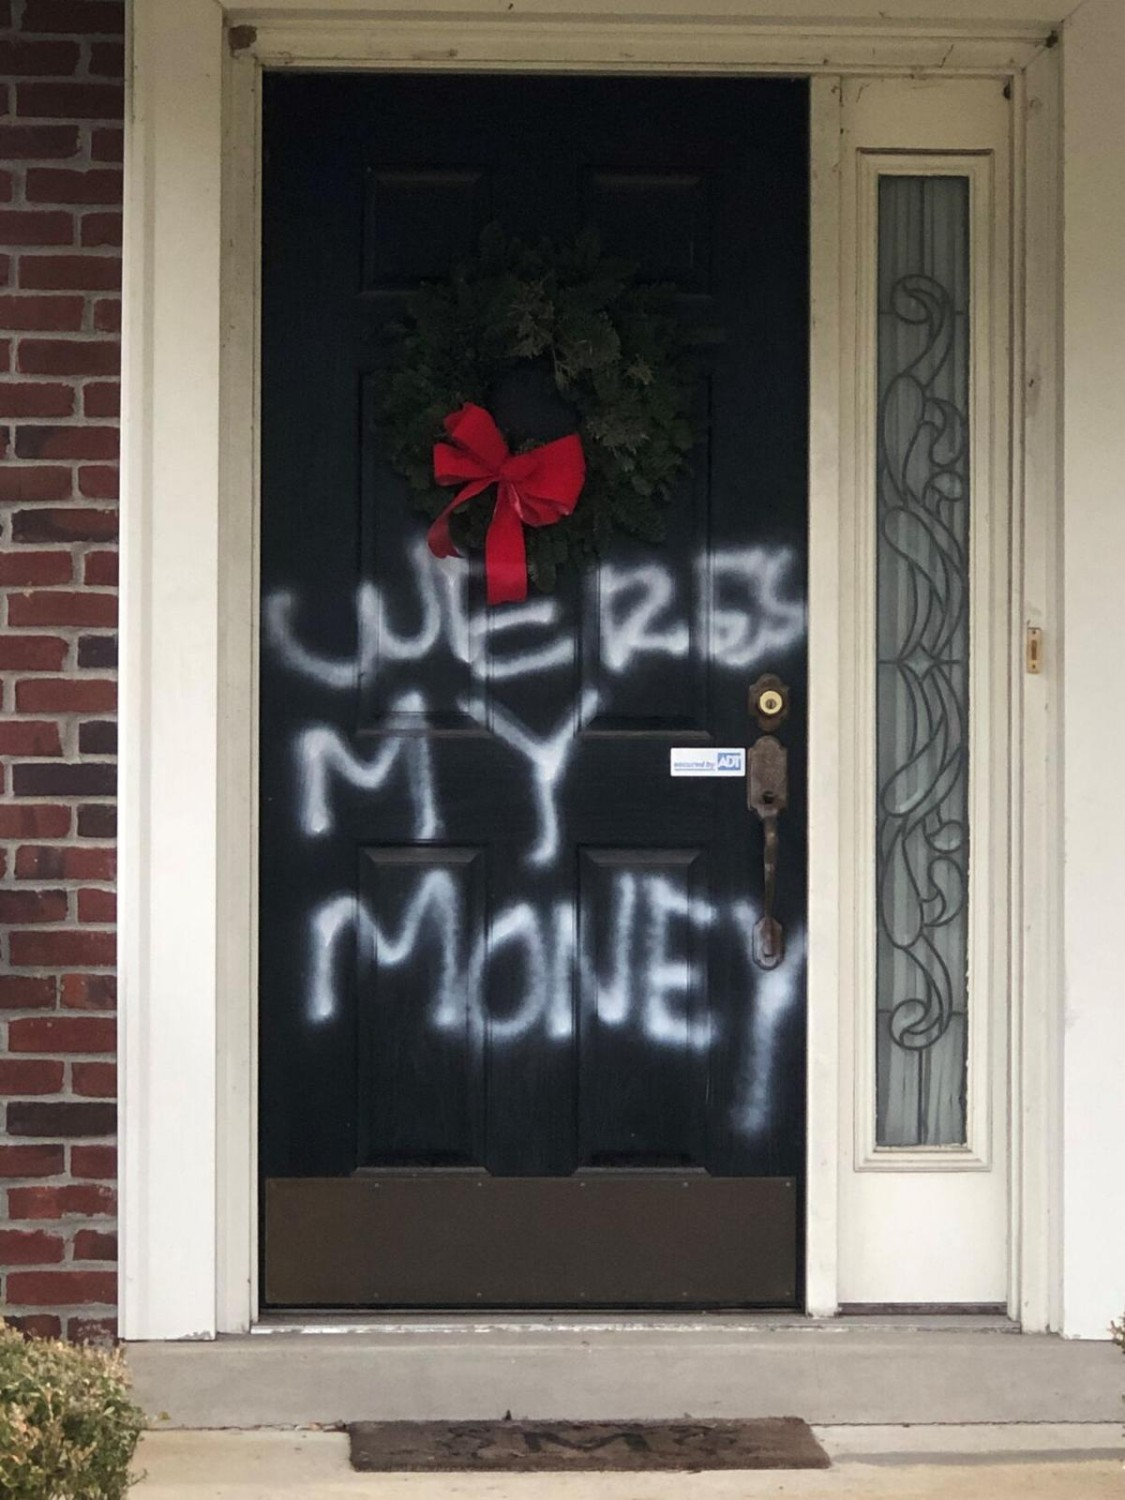
\includegraphics[width=1\textwidth]{images/vandalism.jpg}
  \caption{Akt wandalizmu na drzwiach senatora}
  \label{fig:vandalism}
\end{figure} 

W lipcu 2020 roku fani Taylor Swift zaczęli atakować krytyczkę muzyczną Jillian Mapes po tym, jak opublikowała recenzję albumu Folklore, która ich zdaniem nie była wystarczająco pochlebna. Wkrótce po publikacji recenzji w internecie zaczęły krążyć prywatne dane Mapes, w tym jej adres domowy, numery telefonów oraz zdjęcia jej i jej domu.
Już godzinę po pojawieniu się recenzji zaczęła otrzymywać telefony m.in. o drugiej w nocy oraz groźby przez Twittera, w tym nawoływania do „spalenia jej domu”.
Jillian odpowiedziała na ataki we wpisie na Twitterze, pisząc, że dostaje wiadomości pełne nienawiści, ale mimo strachu, jaki wywołała sytuacja, jest bezpieczna i trzyma się dobrze.

\subsection{Oszustwa socjotechniczne i internetowe}
\subsubsection{Opis zagrożenia}
Ujawnione dane są wykorzystywane do:
\begin{itemize}
  \item phishingu (fałszywe e-maile i strony),
  \item spear-phishingu (ukierunkowane ataki na konkretną osobę),
  \item vishingu (oszustwa telefoniczne),
  \item przekonywania ofiar do ujawnienia loginów i haseł.
\end{itemize}

\subsubsection{Przykłady z życia}
W 2020 r. grupa atakujących uzyskała dostęp do systemów Twittera, podszywając się pod pracowników i kradnąc dane do kont znanych osób.\\

Guy Babcock został niesłusznie oskarżony w internecie o pedofilię i złodziejstwo. Fałszywe wpisy na różnych forach zarzucały Babcockowi i jego rodzinie przestępstwa seksualne i kradzieże. Jego udostepnionych w internecie dane, czyli zdjęcia, miejsce pracy, dane kontaktowe z LinkedIna i Facebooka umożliwiły oszustom wiarygodne przedstawienie jego osoby i jego rodziny jako pedofila oraz złodziei, w postaci wpisów a forum. Wkrótce jego zdjęcia zaczęły krążyć w internecie z podpisem pedofila. Mężczyzna i jego rodzina zaczęli bać się o swoje kariery, reputację i o przyszłość swoich dzieci. I chociaż powstał nawet prostujący te informacje artykuł w magazynie ,,New York Times", to rodzina wciąż boi się o swoje bezpieczeństwo i dobre mniemanie.

\begin{figure}
  \centering
  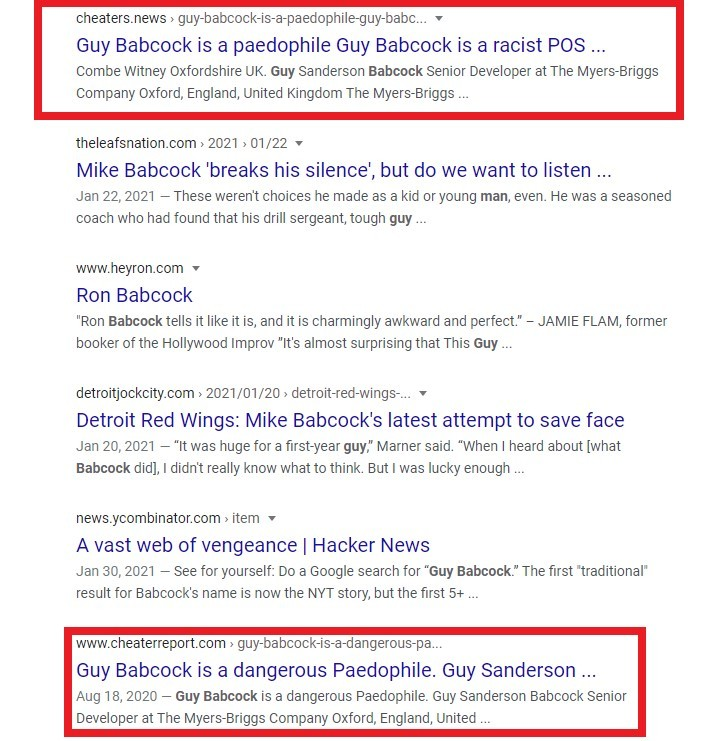
\includegraphics[width=1\textwidth]{images/pedophile.jpg}
  \caption{Fałszywe wpisy oskarżające o pedofilię}
  \label{fig:pedophile}
\end{figure} 

\subsection{Konsekwencje reputacyjne}
\subsubsection{Opis zagrożenia}
Dla osób publicznych, pracowników wysokiego szczebla lub właścicieli firm, ujawnienie danych może prowadzić do:
\begin{itemize}
\item utracenia zaufania klientów i partnerów,
\item negatywnego rozgłosu medialnego
\item trudności w znalezieniu nowej pracy lub rozwijaniu kariery.
\end{itemize}
\subsubsection{Przykłady z życia}
Wyciek danych w firmach takich jak Proofpoint, Apple czy Google nadszarpnął ich wizerunek jako liderów w dziedzinie innowacji i bezpieczeństwa.\\

Facebook był w 2011 roku cytowany w 33\% spraw rozwodowych. Wskazuje to na to, że treści udostepniane w internecie mogą być wykorzystywane przeciwko nam, jako dowody w sprawach sądowych.\\

W wyniku mylnej identyfikacji mężczyzny z nagrania z zamieszek na Kapitolu w 2021 roku, internauci uznali, że to David Quintavalle zabił policjanta. Pan David miał udostępniony w internecie swoje imię, nazwisko, stare zdjęcia, adres domowy. W efekcie doprowadziło to do gróźb, nękań, media przed domem, policyjna ochrona, trwałe powiązanie nazwiska z fałszywym oskarżeniem. Musiał wynająć prawnika, który musiał mu pomóc odbudować jego dobre imię, chociaż bardzo trudno było w pełni pozbyć się nękań.

\begin{figure}
  \centering
  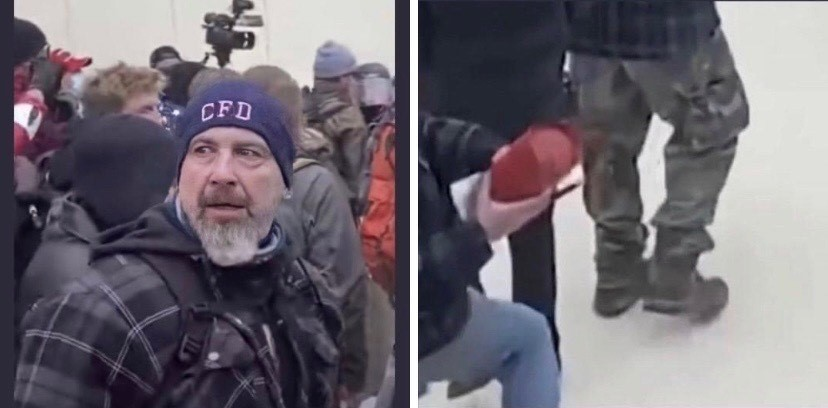
\includegraphics[width=1\textwidth]{images/david.jpg}
  \caption{Fragment nagrania zamieszek na Kapitolu}
  \label{fig:david}
\end{figure} 

\subsection{Odpowiedzialność prawna}
\subsubsection{Opis zagrożenia}
Udostępnianie danych bez zgody lub ich niewłaściwe zabezpieczenie może skutkować:
\begin{itemize}
\item pozwami cywilnymi ze strony poszkodowanych osób,
\item karami finansowymi za naruszenie przepisów o ochronie danych (np. RODO/GDPR),
\item odpowiedzialnością dyscyplinarną lub karną.
\end{itemize}

\subsubsection{Przykłady z życia}
Microsoft mógłby zostać ukarany grzywną do 20 mln euro za wyciek danych z systemów GitHub, gdyby doszło do naruszenia danych klientów z UE.\\

Japończyk Hibiki Sato użył zdjęć z mediów społecznościowych i na podstawie refleksów w oczach i Google Street View, by odnaleźć kobietę i ją zaatakować. Po tym wydarzeniu kobieta musiała się długi czas zmagać z traumą, natomiast stalker poniósł odpowiedzialność prawną - skazanie na 30 miesięcy pozbawienia wolności w 2020 roku.
\begin{figure}
  \centering
  
\includegraphics[width=1\textwidth]{images/stalker.jpg}
  \caption{Hibiki Sato}
  \label{fig:stalker}
\end{figure}

Yue Chen, pacjent z rakiem w IV stadium, który oskarżył swoich lekarzy o traktowanie go jak „małpę laboratoryjną”, odnalazł ich domowe adresy w rejonie zatoki San Francisco i planował ich zamordowanie.
31 maja 2017 roku członkowie rodziny Chen'a zgłosili jego zaginięcie. Gdy policja przybyła na miejsce, znalazła notatkę, w której mężczyzna napisał, że „musi dziś zabić tych lekarzy, ponieważ są źli”.
Na szczęście Chen zgubił się i nie odnalazł żadnego z domów lekarzy. Policja zatrzymała go, gdy próbował wrócić do siebie. W jego samochodzie znaleziono dwie naładowane półautomatyczne pistolety, notatnik z ręcznie przepisanymi z Google Maps wskazówkami dojazdu do domów lekarzy oraz białą gumową maskę. Znaleziono również notatkę zatytułowaną „dlaczego zabijam”, w której napisał: „to jest możliwe, jeśli traktujecie ludzi jak zwierzę”.